\documentclass[12pt,letterpaper]{article}
\usepackage{graphicx,textcomp}
\usepackage{natbib}
\usepackage{setspace}
\usepackage{fullpage}
\usepackage{color}
\usepackage[reqno]{amsmath}
\usepackage{amsthm}
\usepackage{fancyvrb}
\usepackage{amssymb,enumerate}
\usepackage[all]{xy}
\usepackage{endnotes}
\usepackage{lscape}
\newtheorem{com}{Comment}
\usepackage{float}
\usepackage{hyperref}
\newtheorem{lem} {Lemma}
\newtheorem{prop}{Proposition}
\newtheorem{thm}{Theorem}
\newtheorem{defn}{Definition}
\newtheorem{cor}{Corollary}
\newtheorem{obs}{Observation}
\usepackage[compact]{titlesec}
\usepackage{dcolumn}
\usepackage{tikz}
\usetikzlibrary{arrows}
\usepackage{multirow}
\usepackage{xcolor}
\newcolumntype{.}{D{.}{.}{-1}}
\newcolumntype{d}[1]{D{.}{.}{#1}}
\definecolor{light-gray}{gray}{0.65}
\usepackage{url}
\usepackage{listings}
\usepackage{color}

\definecolor{codegreen}{rgb}{0,0.6,0}
\definecolor{codegray}{rgb}{0.5,0.5,0.5}
\definecolor{codepurple}{rgb}{0.58,0,0.82}
\definecolor{backcolour}{rgb}{0.95,0.95,0.92}

\lstdefinestyle{mystyle}{
	backgroundcolor=\color{backcolour},   
	commentstyle=\color{codegreen},
	keywordstyle=\color{magenta},
	numberstyle=\tiny\color{codegray},
	stringstyle=\color{codepurple},
	basicstyle=\footnotesize,
	breakatwhitespace=false,         
	breaklines=true,                 
	captionpos=b,                    
	keepspaces=true,                 
	numbers=left,                    
	numbersep=5pt,                  
	showspaces=false,                
	showstringspaces=false,
	showtabs=false,                  
	tabsize=2
}
\lstset{style=mystyle}
\newcommand{\Sref}[1]{Section~\ref{#1}}
\newtheorem{hyp}{Hypothesis}

\title{House Price Presentation}
\date{November 30, 2022}
\author{Ruairí Hallissey, Lilly Rice, and Tianxin 'Caesar' Zhang}

\begin{document}
	\maketitle
\newpage
\section{Initial Model}
\begin{table}[!htbp] \centering 
	\caption{} 
	\label{} 
	\begin{tabular}{@{\extracolsep{5pt}}lc} 
		\\[-1.8ex]\hline 
		\hline \\[-1.8ex] 
		& \multicolumn{1}{c}{\textit{Dependent variable:}} \\ 
		\cline{2-2} 
		\\[-1.8ex] & AdjSalePrice \\ 
		\hline \\[-1.8ex] 
		BldgGrade & 112,748.800$^{***}$ \\ 
		& (2,467.120) \\ 
		& \\ 
		SqFtTotLiving & 182.260$^{***}$ \\ 
		& (3.184) \\ 
		& \\ 
		Constant & $-$680,074.400$^{***}$ \\ 
		& (14,597.660) \\ 
		& \\ 
		\hline \\[-1.8ex] 
		Observations & 20,340 \\ 
		R$^{2}$ & 0.532 \\ 
		Adjusted R$^{2}$ & 0.532 \\ 
		Residual Std. Error & 264,989.900 (df = 20337) \\ 
		F Statistic & 11,549.010$^{***}$ (df = 2; 20337) \\ 
		\hline 
		\hline \\[-1.8ex] 
		\textit{Note:}  & \multicolumn{1}{r}{$^{*}$p$<$0.1; $^{**}$p$<$0.05; $^{***}$p$<$0.01} \\ 
	\end{tabular} 
\end{table}

\newpage
\section{Adding Zip Group}
\begin{figure}[!h]
	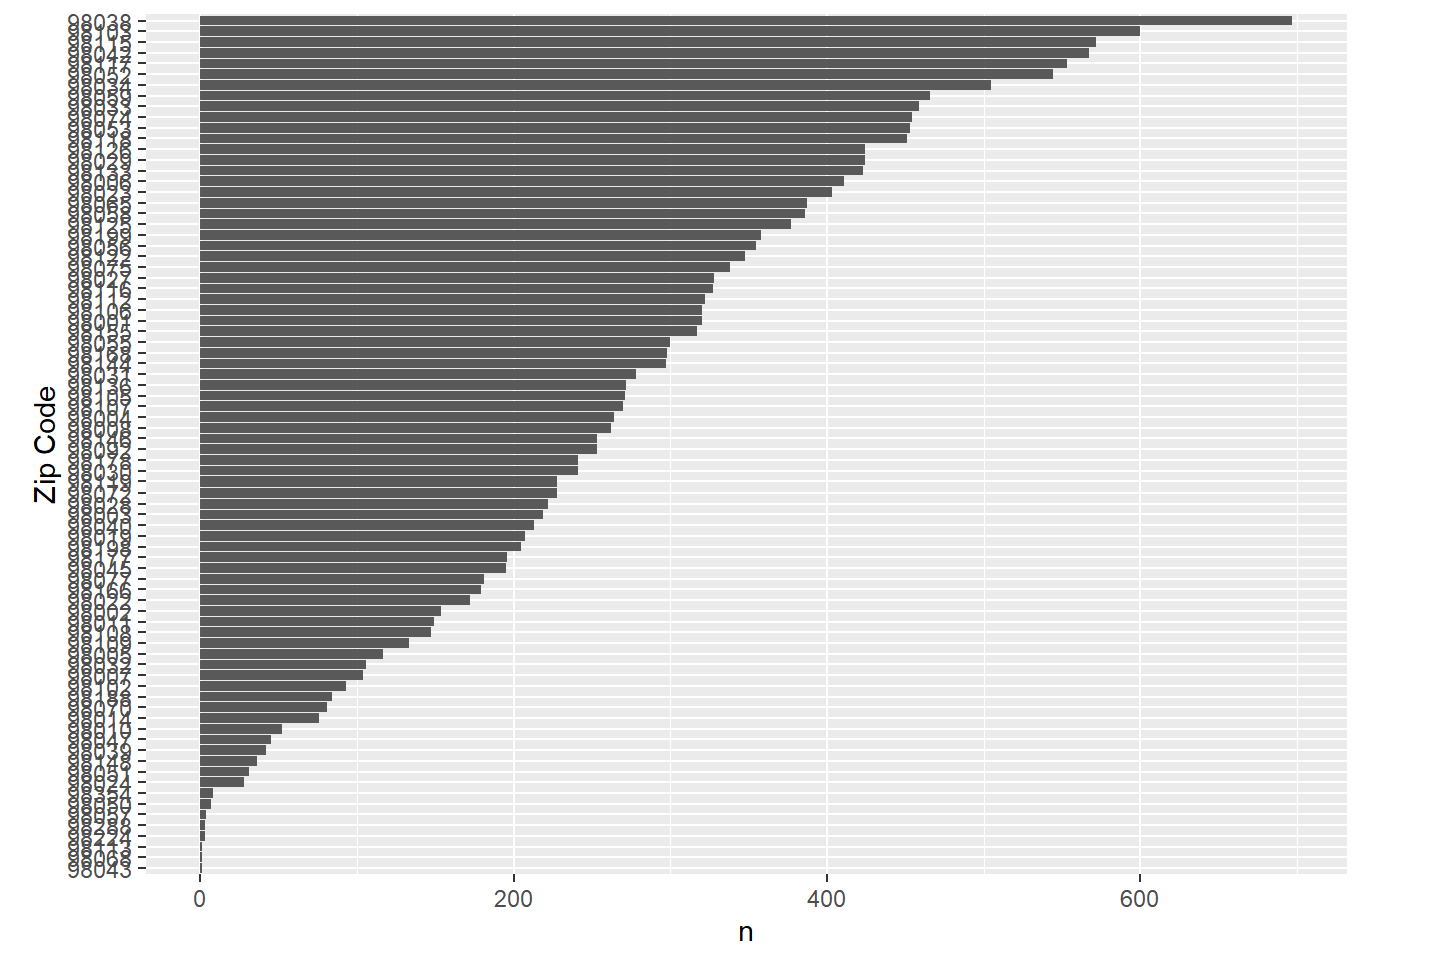
\includegraphics[width= 150mm]{image}
	\caption{\small \sl Zip codes arranged by price.\label{fig:Stupendous}} 
\end{figure}

\newpage
\begin{table}[!htbp] \centering 
	\caption{} 
	\label{} 
	\begin{tabular}{@{\extracolsep{5pt}}lcc} 
		\\[-1.8ex]\hline 
		\hline \\[-1.8ex] 
		& \multicolumn{2}{c}{\textit{Dependent variable:}} \\ 
		\cline{2-3} 
		\\[-1.8ex] & AdjSalePrice & AdjSalePrice \\ 
		\\[-1.8ex] & (1) & (2)\\ 
		\hline \\[-1.8ex] 
		BldgGrade & 112,748.800$^{***}$ &  \\ 
		& (2,467.120) &  \\ 
		& & \\ 
		SqFtTotLiving & 182.260$^{***}$ &  \\ 
		& (3.184) &  \\ 
		& & \\ 
		SqFtTotLiving &  & 187.401$^{***}$ \\ 
		&  & (3.171) \\ 
		& & \\ 
		BldgGrade &  & 115,248.000$^{***}$ \\ 
		&  & (2,450.739) \\ 
		& & \\ 
		ZipGroup &  & 26,362.780$^{***}$ \\ 
		&  & (1,435.057) \\ 
		& & \\ 
		Constant & $-$680,074.400$^{***}$ & $-$790,502.900$^{***}$ \\ 
		& (14,597.660) & (15,676.660) \\ 
		& & \\ 
		\hline \\[-1.8ex] 
		Observations & 20,340 & 20,340 \\ 
		R$^{2}$ & 0.532 & 0.539 \\ 
		Adjusted R$^{2}$ & 0.532 & 0.539 \\ 
		Residual Std. Error & 264,989.900 (df = 20337) & 262,824.600 (df = 20336) \\ 
		F Statistic & 11,549.010$^{***}$ (df = 2; 20337) & 7,939.216$^{***}$ (df = 3; 20336) \\ 
		\hline 
		\hline \\[-1.8ex] 
		\textit{Note:}  & \multicolumn{2}{r}{$^{*}$p$<$0.1; $^{**}$p$<$0.05; $^{***}$p$<$0.01} \\ 
	\end{tabular} 
\end{table}

\newpage
\section{Transformations}
\begin{figure}[!h]
	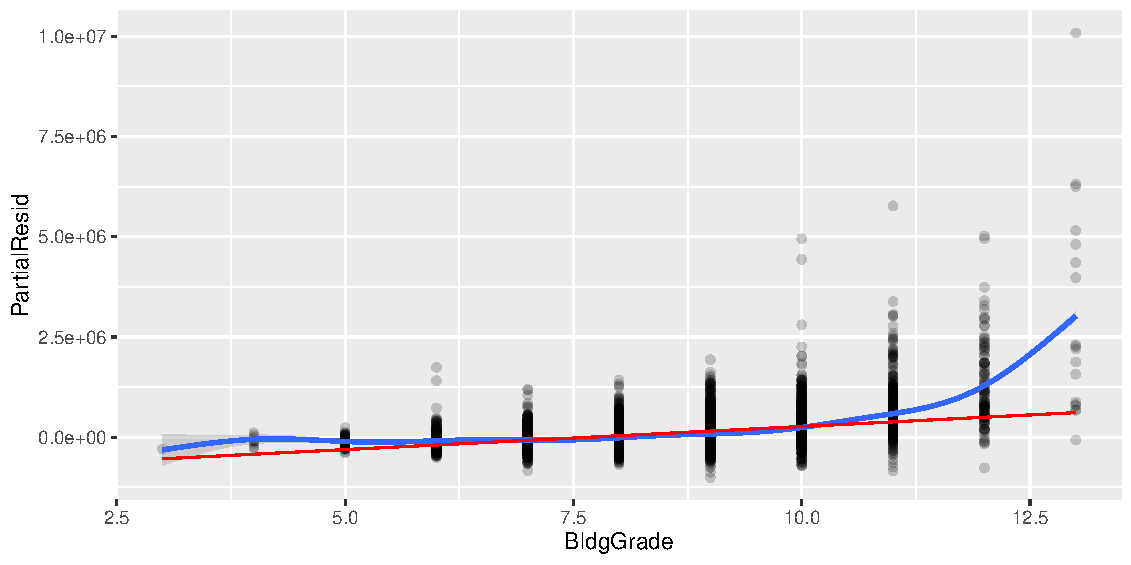
\includegraphics[width= 150mm]{BldgPartialRegRplot}
	\caption{\small \sl Partial residual plot for building grade.\label{fig:Stupendous}} 
\end{figure}

\begin{figure}[!h]
	\includegraphics[width= 150mm]{BlG^2ParRegRplot}
	\caption{\small \sl Partial residual plot for building grade squared.\label{fig:Stupendous}} 
\end{figure}

\newpage
\section*{Transformations}
\begin{figure}[!h]
	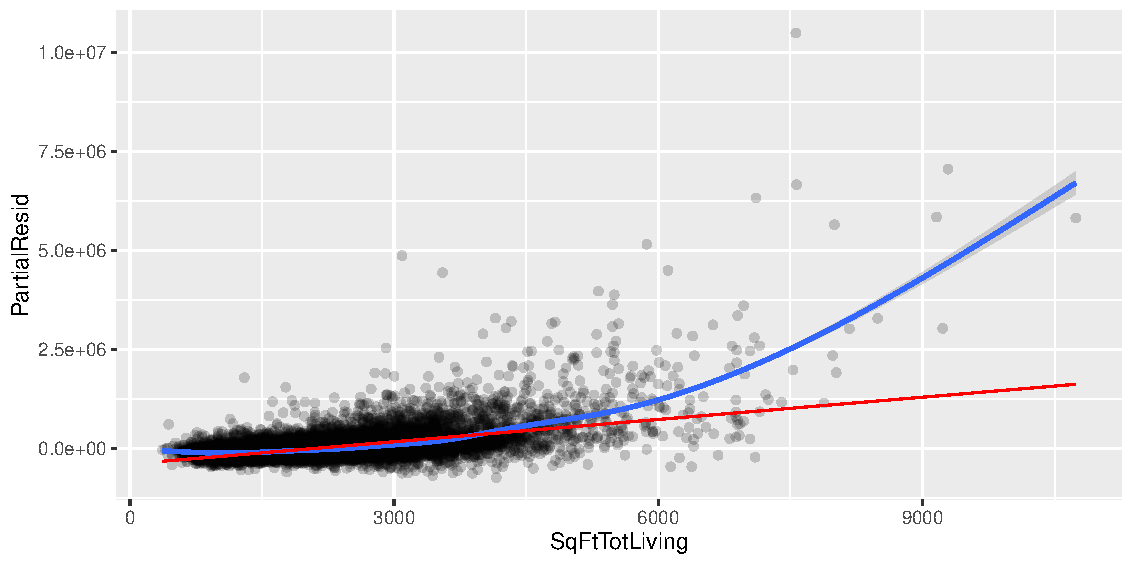
\includegraphics[width= 150mm]{SqrftlParRegRplot}
	\caption{\small \sl Partial residual for square foot to living.\label{fig:Stupendous}} 
\end{figure}

\begin{figure}[!h]
	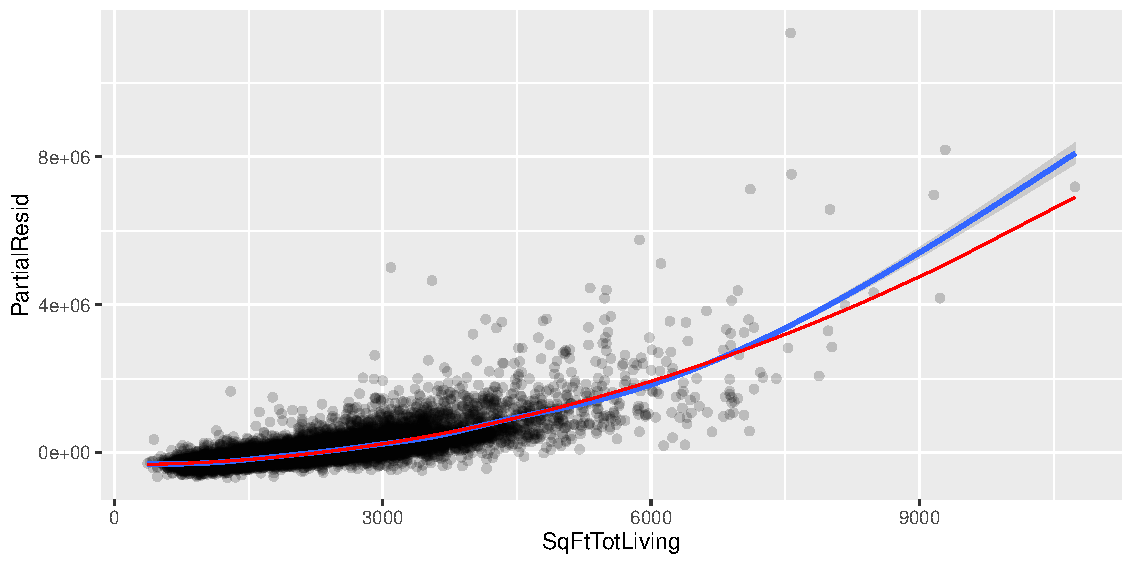
\includegraphics[width= 150mm]{SqrfTL^2ParRegRplot}
	\caption{\small \sl Partial residual for square foot to living squared.\label{fig:Stupendous}} 
\end{figure}

\newpage
\section*{Final Model}
\begin{table}[!htbp] \centering 
	\footnotesize
	\caption{} 
	\label{} 
	\begin{tabular}{@{\extracolsep{5pt}}lccc} 
		\\[-1.8ex]\hline 
		\hline \\[-1.8ex] 
		& \multicolumn{3}{c}{\textit{Dependent variable:}} \\ 
		\cline{2-4} 
		\\[-1.8ex] & AdjSalePrice & \multicolumn{2}{c}{AdjSalePrice} \\ 
		\\[-1.8ex] & (1) & (2) & (3)\\ 
		\hline \\[-1.8ex] 
		BldgGrade & 112,748.800$^{***}$ &  &  \\ 
		& (2,467.120) &  &  \\ 
		& & & \\ 
		SqFtTotLiving & 182.260$^{***}$ &  &  \\ 
		& (3.184) &  &  \\ 
		& & & \\ 
		I(SqFtTotLiving$\hat{\mkern6mu}$2) &  &  & 0.045$^{***}$ \\ 
		&  &  & (0.001) \\ 
		& & & \\ 
		SqFtTotLiving &  & 187.401$^{***}$ & $-$84.272$^{***}$ \\ 
		&  & (3.171) & (7.004) \\ 
		& & & \\ 
		BldgGrade &  & 115,248.000$^{***}$ & $-$271,926.800$^{***}$ \\ 
		&  & (2,450.739) & (15,224.020) \\ 
		& & & \\ 
		I(BldgGrade$\hat{\mkern6mu}$2) &  &  & 24,630.760$^{***}$ \\ 
		&  &  & (939.220) \\ 
		& & & \\ 
		ZipGroup &  & 26,362.780$^{***}$ & 21,096.620$^{***}$ \\ 
		&  & (1,435.057) & (1,298.708) \\ 
		& & & \\ 
		Constant & $-$680,074.400$^{***}$ & $-$790,502.900$^{***}$ & 1,044,462.000$^{***}$ \\ 
		& (14,597.660) & (15,676.660) & (58,097.830) \\ 
		& & & \\ 
		\hline \\[-1.8ex] 
		Observations & 20,340 & 20,340 & 20,340 \\ 
		R$^{2}$ & 0.532 & 0.539 & 0.625 \\ 
		Adjusted R$^{2}$ & 0.532 & 0.539 & 0.625 \\ 
		Residual Std. Error & 264,989.900 (df = 20337) & 262,824.600 (df = 20336) & 237,271.500 (df = 20334) \\ 
		F Statistic & 11,549.010$^{***}$ (df = 2; 20337) & 7,939.216$^{***}$ (df = 3; 20336) & 6,768.416$^{***}$ (df = 5; 20334) \\ 
		\hline 
		\hline \\[-1.8ex] 
		\textit{Note:}  & \multicolumn{3}{r}{$^{*}$p$<$0.1; $^{**}$p$<$0.05; $^{***}$p$<$0.01} \\ 
	\end{tabular} 
\end{table}

\end{document}